\section{Calculation of Physical Properties} \label{sec:calculation_of_physical_properties}
\noindent
KitFox provides several API functions to invoke the calculation of physical models.

\subsection{Power Calculation} \label{subsec:power_calculation}
\noindent
Dynamic energy is calculated with respect to access counters that have to be collected from microarchitecture simulators (refer to Section \ref{subsec:counter} for counter definition). 
Per-access energies of distinct access types are estimated by the physical models and multiplied with the counters of corresponding access types (refer to Section \ref{subsec:unit_energy} for unit energy definition). 
The calculated power result is stored in the data queue of the pseudo component that can be probed by a queue operation functions $|pull\_data|$.
{
\fontsize{10pt}{11pt}\selectfont
\begin{alltt}
void calculate_power(Comp_ID ComponentID, Second Time, Second Period, counter_t Counter);
\end{alltt}
}

\noindent
This function can be called with the pseudo components linked to one of the following physical models.
\begin{itemize}
\item{DRAMSim2} \vspace*{-5pt}\leavevmode
\item{DSENT} \vspace*{-5pt}\leavevmode
\item{IntSim} \vspace*{-5pt}\leavevmode
\item{McPAT}
\end{itemize}

\noindent
$|calculate_power|$ function performs the following operations.
{
\fontsize{10pt}{11pt}\selectfont
\begin{alltt}
energy.dynamic = unit_energy.baseline * period * clock_frequency;
energy.dynamic += unit_energy.switching * counter.switching;
energy.dynamic += unit_energy.read * counter.read;
energy.dynamic += unit_energy.write * counter.write;
energy.dynamic += unit_energy.read_tag * counter.read_tag;
energy.dynamic += unit_energy.write_tag * counter.write_tag;
energy.dynamic += unit_energy.search * counter.search;
energy.dynamic += unit_energy.precharge * counter.precharge;
energy.dynamic += unit_energy.background_open_page_high * counter.background_open_page_high;
energy.dynamic += unit_energy.background_open_page_low * counter.background_open_page_low;
energy.dynamic += unit_energy.background_closed_page_high * counter.background_closed_page_high;
energy.dynamic += unit_energy.background_closed_page_low * counter.background_closed_page_low;
energy.leakage = unit_energy.leakage * period * clock_frequency;
energy.total = energy.dynamic + energy.leakage;
power = energy / period;
\end{alltt}
}

\subsection{Temperature Calculation} \label{subsec:temperature_calculation}
\noindent
Temperature is calculated based on the power distribution of thermal blocks (i.e., floorplans, thermal grid cells) on the die. 
This function first synchronizes the power data of pseudo components. 
When $|DoPowerSync|$ = $|false|$, KitFox assumes that the power data are already synchronized and skips this process. 
If pseudo components have asynchronous power data, the simulation terminates with an error message. 
After calculating the temperature, pseudo components that are designated as floorplans have updated temperature values in the data queues. 
Temperature data are then synchronized across pseudo components. 
It is assumed that the temperature is uniform within the floorplan by assuming that no further placement information is available. 
All the descendent components of the floorplan are updated with the same temperature.
{
\fontsize{10pt}{11pt}\selectfont
\begin{alltt}
void calculate_temperature(Comp_ID ComponentID, Second Time, Second Period, bool DoPowerSync);
\end{alltt}
}
\noindent
This function can be called at pseudo components associated with one of the following physical models.
\begin{itemize}
\item{3D-ICE} \vspace*{-5pt}\leavevmode
\item{HotSpot} \vspace*{-5pt}\leavevmode
\item{Microfluidics}
\end{itemize}

\subsection{Failure Rate (Reliability) Calculation} \label{subsec:failure_rate_calculation}
\noindent
Failure rates are calculated based on the temperature, voltage, and clock frequency of modeled blocks. 
These variables must be updated before calling the reliability calculation function. 
When $|DoDataSync|$ = $|false|$, KitFox skips the synchronization process. 
Note that temperature ($|KITFOX_DATA_TEMPERATURE|$) is stored in the closed queue that requires data insertion at every sampling point, which means that $|calculate\_temperature|$ function must be called prior to this function. 
On the other hand, voltage ($|KITFOX_DATA_VOLTAGE|$) and clock frequency($|KITFOX_DATA_CLOCK_FREQUENCY|$) are stored in open queues that return the data for the requests between [$t$, $\infty$), where $t$ is the time that the last values were inserted. 
If voltage and frequency are not updated before calling this function but are supposed to be scaled, then this function can inadvertently calculate the failure rate based on the old voltage and frequency values. 
However, it is rare for this case to occur since most control decision (e.g., DVFS) are made after physical calculations are all completed.
The following function is called at the pseudo component associated with the $|failure|$ physical model. 
{
\fontsize{10pt}{11pt}\selectfont
\begin{alltt}
void calculate_failure_rate(Comp_ID ComponentID, Second Time, Second Period, bool DoDataSync);
\end{alltt}
}

\noindent
When this function is invoked, what is actually stored in the data queue is $\lambda t$ value, where $\lambda t = \sum_{i=1}^{N} \lambda_{i} (t_{i} - t_{i-1})$ based on the exponential distribution model. 
$i$ is the index of $N$ sampling points; $t_{N}$ is the current time, and $t_{N}-t_{N-1}$ is the last sampling period. 
$\lambda_{i}$ is the transient failure rate of $i^{\text{th}}$ sampling point. 
The mean-time-to-failure (MTTF) can be calculated as $\frac{t}{\lambda t}$ indicating the expected lifetime based on the cumulative calculation of transient failure rates.

\subsection{Calculation Sequence} \label{subsec:calculation_sequence}
\noindent
Processor physical properties are dynamically interacting with each other, creating dependencies as illustrated in Figure \ref{fig:interactive_simulation}. 
It is critical to follow the exact sequence of calculations in order to correctly model the physical interactions chain as well as not to break the simulations.

\begin{figure}[h]
\centering
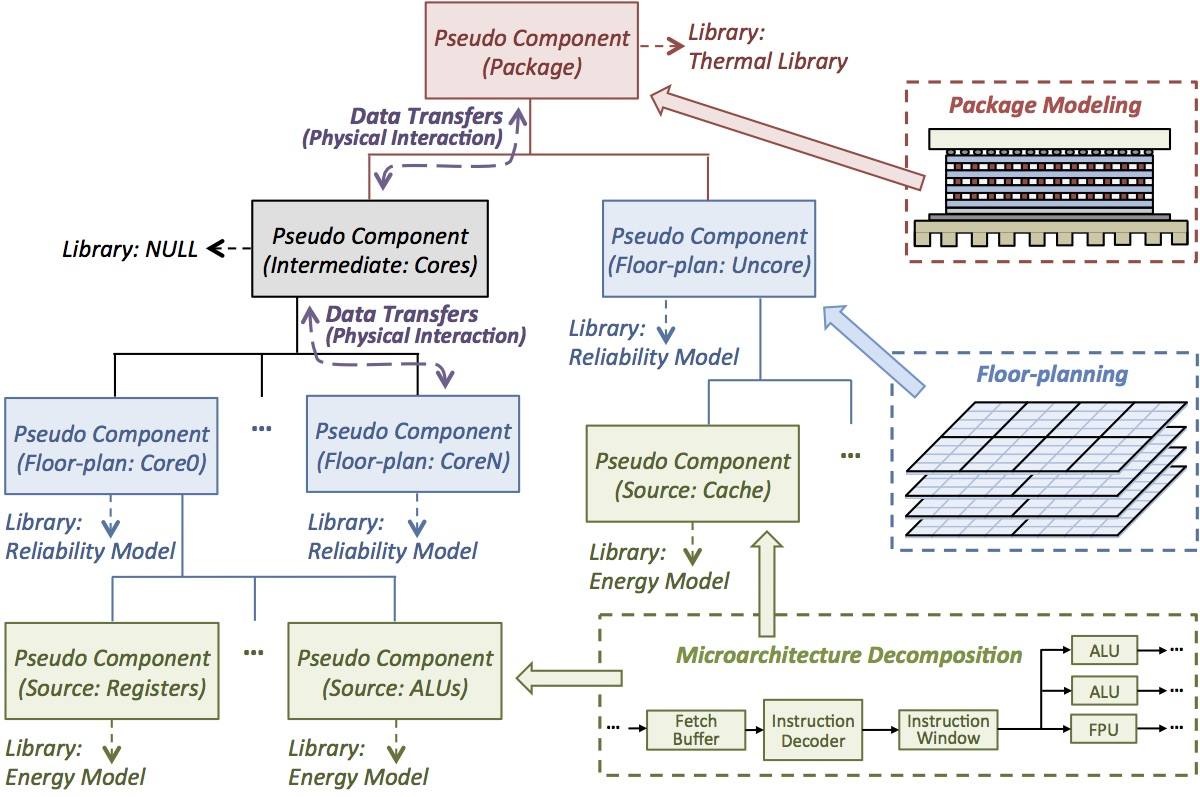
\includegraphics[width=0.6 \textwidth]{figures/kitfox_hierarchy.jpg}
\caption{A processor is represented as the \emph{pseudo component hierarchy} in KitFox framework. Pseudo components are physically defined units where associated libraries estimate physical phenomena. Physical interactions are emulated by transferring data between the data queues of pseudo components.}
\label{fig:kitfox_hierarchy}
\end{figure}

\noindent
The following shows an example of stepwise function calls to perform the physics chain shown in Figure \ref{fig:interactive_simulation}.

{
\fontsize{10pt}{11pt}\selectfont
\begin{alltt}
while (program runs) \{
    clock_cycle++;
    Do \{architecture timing simulation and counters collection\}
    
    if (@sampling point) \{
        Second time = get_current_time();
        Second period = get_sampling_interval();
        
        /* Calculate power for all source components with power models */
        for (all source components with power models) \{
            kitfox->calculate_power(src_comp_id, time, period, src_comp_counters);
        \}
        
        /* Calculate temperature at the component with thermal model. 
        Power-temperature dependency is internally captured here. */
        kitfox->calculate_temperature(package_cmp_id, time, period, /*DoPowerSync*/true);
        
        /* Calculate failure rate for all components with reliability models. 
        Temperature-voltage-frequency-reliability dependency is captured here. */
        for (all components (e.g., floor-plans) with reliability models) \{
            kitfox->calculate_failure_rate(flp_comp_id, time, period, /*DoDataSync*/true);
        \}
        
        /* Probe any components of interest and retrieve the data */
        Kelvin core0_temperature;
        int error_code = kitfox->pull_data(core0_id, time, period,\(\backslash\)
                         KITFOX_DATA_TEMPERATURE, &core0_temperature);
        assert(error_code == KITFOX_QUEUE_ERROR_NONE);
        
        /* Apply execution control (e.g., frequency scaling) */
        if(core0_temperature > thermal_threshold) \{
            Hertz P4_state_freq = 1.0e9; // 1GHz
            error_code = kitfox->push_and_synchronize_data(core0_id, time, period,\(\backslash\)
                         KITFO_DATA_CLOCK_FREQUENCY, &P4_state_freq);
            assert(error_code == KITFOX_QUEUE_ERROR_NONE);
        \}
    \}
\}
\end{alltt}
}
 
